\documentclass[a4paper]{article}
\usepackage{svn-multi}
% Version control information:
\svnidlong
{$HeadURL: https://practicas-derive.googlecode.com/svn/trunk/aplicaciones_derivada.tex $}
{$LastChangedDate: 2008-11-13 12:37:02 +0100 (jue, 13 nov 2008) $}
{$LastChangedRevision: 3 $}
{$LastChangedBy: asalber $}
\svnid{$Id: aplicaciones_derivada.tex 3 2008-11-13 11:37:02Z asalber $}
\pdfinfo{/CreationDate (D:\svnpdfdate)}
\svnRegisterAuthor{alf}{Alfredo Sánchez Alberca}

\usepackage[spanish]{babel}
\usepackage[utf8x]{inputenc}
\usepackage{amsmath}
\usepackage{macros}
\usepackage[dvips]{graphicx}
\usepackage{enumitem}
\usepackage{subfigure}
\usepackage[small,bf]{caption2}
\usepackage[top=3cm, bottom=3cm, left=2.54cm, right=2.54cm]{geometry}
\usepackage{fancyhdr}
\pagestyle{fancy}

\lhead{\textsc{Universidad San Pablo CEU}} \rhead{\textsl{\textsf{Departamento de Métodos Cuantitativos}}}
\renewcommand{\headrulewidth}{0pt}
\renewcommand{\floatpagefraction}{.8}
\renewcommand{\textfraction}{.1}
\setcaptionwidth{\textwidth} \addtolength{\captionwidth}{-40pt}
\captionstyle{indent} \setlength\captionindent{\parindent}

\makeatletter
\let\savees@listquot\es@listquot
\def\es@listquot{\protect\savees@listquot}
\makeatletter

\begin{document}
\sloppy
\practica{Práctica de Cálculo con Derive}{Aplicaciones de la Derivada}

\bigskip
\section*{Fundamentos Teóricos}
El estudio del signo de la derivada de una función resulta de gran ayuda en el estudio del crecimiento de la función, así como en la determinación de los extremos relativos de la misma. De igual modo, el estudio del signo de la segunda derivada resulta útil en el estudio de la concavidad de la función. En esta práctica también se muestran varios teoremas importantes relacionados con la derivada.

\subsection*{Estudio del crecimiento de una función}
Una función $f(x)$ es \emph{creciente} en un intervalo $I$ si $\forall\, x_1, x_2 \in I$ tales que $x_1<x_2$ se verifica que $f(x_1)\leq f(x_2)$. 

Del mismo modo, se dice que una función $f(x)$ es \emph{decreciente} en un intervalo $I$ si $\forall\, x_1, x_2 \in I$ tales que $x_1<x_2$ se verifica que $f(x_1)\geq f(x_2)$. En la figura~\ref{g:crecimiento} se muestran estos conceptos.

\begin{figure}[h!]
\centering
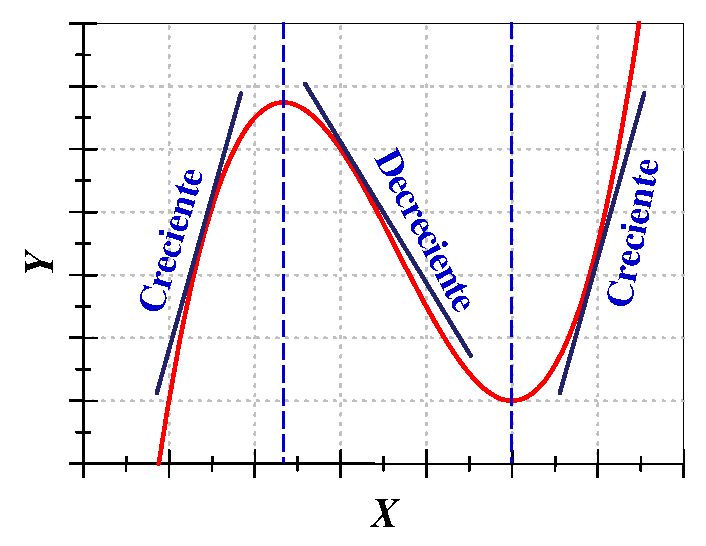
\includegraphics[scale=0.6]{crecimiento}
\caption{Intervalos de crecimiento y decrecimiento de una función.}
\label{g:crecimiento}
\end{figure}

Si $f$ es una función derivable en el intervalo $I$, el signo de la derivada puede utilizarse para estudiar el crecimiento de la función ya que se cumple:
\begin{itemize}
\item $f$ es creciente en $x_0\in I$, si y sólo si, $f'(x_0)\geq 0$.
\item $f$ es decreciente en $x_0\in I$, si y sólo si, $f'(x_0)\leq 0$.
\end{itemize}

Desde el punto de vista geométrico, esto es evidente, ya en los intervalos donde $f$ es creciente, cualquier recta tangente tiene pendiente positiva, mientras que en los intervalos donde $f$ es decreciente, las tangentes tienen pendiente negativa, tal y como se observa en la figura~\ref{g:crecimiento}.

\subsection*{Determinación de los extremos relativos}
Una función $f(x)$ tiene un \emph{máximo relativo} en $x_0$ si existe un entorno $A$ de $x_0$ tal que $\forall x \in A$ se verifica que $f(x)\leq f(x_0)$.

Una función $f(x)$ tiene un \emph{mínimo relativo} en $x_0$ si existe un entorno $A$ de $x_0$ tal que $\forall x\in A$ se verifica que $f(x)\geq f(x_0)$.

Diremos que la función $f(x)$ tiene un \emph{extremo relativo} en un punto si tiene un \emph{máximo o mínimo relativo} en dicho punto.

Cuando $f$ es una función continua, entonces también se puede definir un extremo relativo como aquel punto donde cambia el crecimiento de la función. Así, un máximo relativo el un punto donde la función pasa de ser creciente a ser decreciente, y un mínimo relativo es un punto donde la función pasa de ser decreciente a ser creciente, tal y como se muestra en la figura~\ref{g:extremos}.

\begin{figure}[h!]
\centering
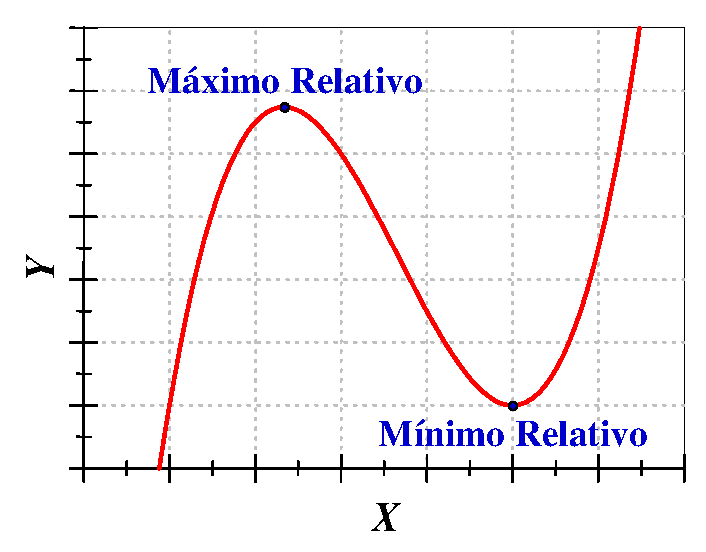
\includegraphics[scale=0.6]{extremos}
\caption{Máximo y mínimo relativo de una función.}
\label{g:extremos}
\end{figure}

Si $f$ tiene un extremo relativo en un punto $x_0$ y existe la derivada en dicho punto, entonces se cumple que $f'(x_0)=0$, es decir, la tangente a la gráfica de $f$ en dicho punto es horizontal (figura~\ref{g:extremos}). El recíproco no es cierto en general, de modo que esta es una condición necesaria pero no suficiente. No obstante, si $f$ es una función derivable en un intervalo $I$, podemos utilizar esta propiedad para detectar los puntos entre los que se encontrarán los extremos relativos del intervalo $I$. Los puntos donde se anula la primera derivada, se conocen como \emph{puntos críticos} y serán candidatos a extremos. Una vez detectados los puntos críticos, para ver si se trata de un extremo relativo o no, basta con estudiar el crecimiento de la función a la izquierda y a la derecha del punto tal y como se indicaba en la sección anterior. Resumiendo, si $f'(x_0)=0$, entonces
\begin{itemize}
\item Si existe un $\delta>0$ tal que $f'(x)>0\ \forall\, x\in (x_0-\delta,x_0)$ (derivada positiva a la izquierda de $x_0$) y $f'(x)<0\ \forall\, x\in (x_0,x_0+\delta)$ (derivada negativa a la derecha de $x_0$), $x_0$ es un máximo relativo.

\item Si existe un $\delta>0$ tal que $f'(x)<0\ \forall\, x\in (x_0-\delta,x_0)$ (derivada negativa a la izquierda de $x_0$) y $f'(x)>0\ \forall\, x\in (x_0,x_0+\delta)$ (derivada positiva a la derecha de $x_0$), $x_0$ es un mínimo relativo.

\item En cualquier otro, $x_0$ es un \emph{punto de inflexión}.
\end{itemize}

\subsection*{Estudio de la concavidad de una función}
Se dice que una función $f(x)$ es \emph{cóncava} en un intervalo $I$ si $\forall\, x_1, x_2 \in I$, el segmento de extremos $(x_1,f(x_1))$ y $(x_2,f(x_2))$ queda por debajo de la gráfica de $f$.

Análogamente se dirá que es \emph{convexa} si el segmento anterior queda por encima de la gráfica de $f$. 

Diremos que la función $f(x)$ tiene un \emph{punto de inflexión} en $x_0$ si en ese punto la función pasa de cóncava a convexa o de convexa a cóncava. Estos conceptos se ilustran en la figura~\ref{g:concavidad}.

\begin{figure}[h!]
\centering
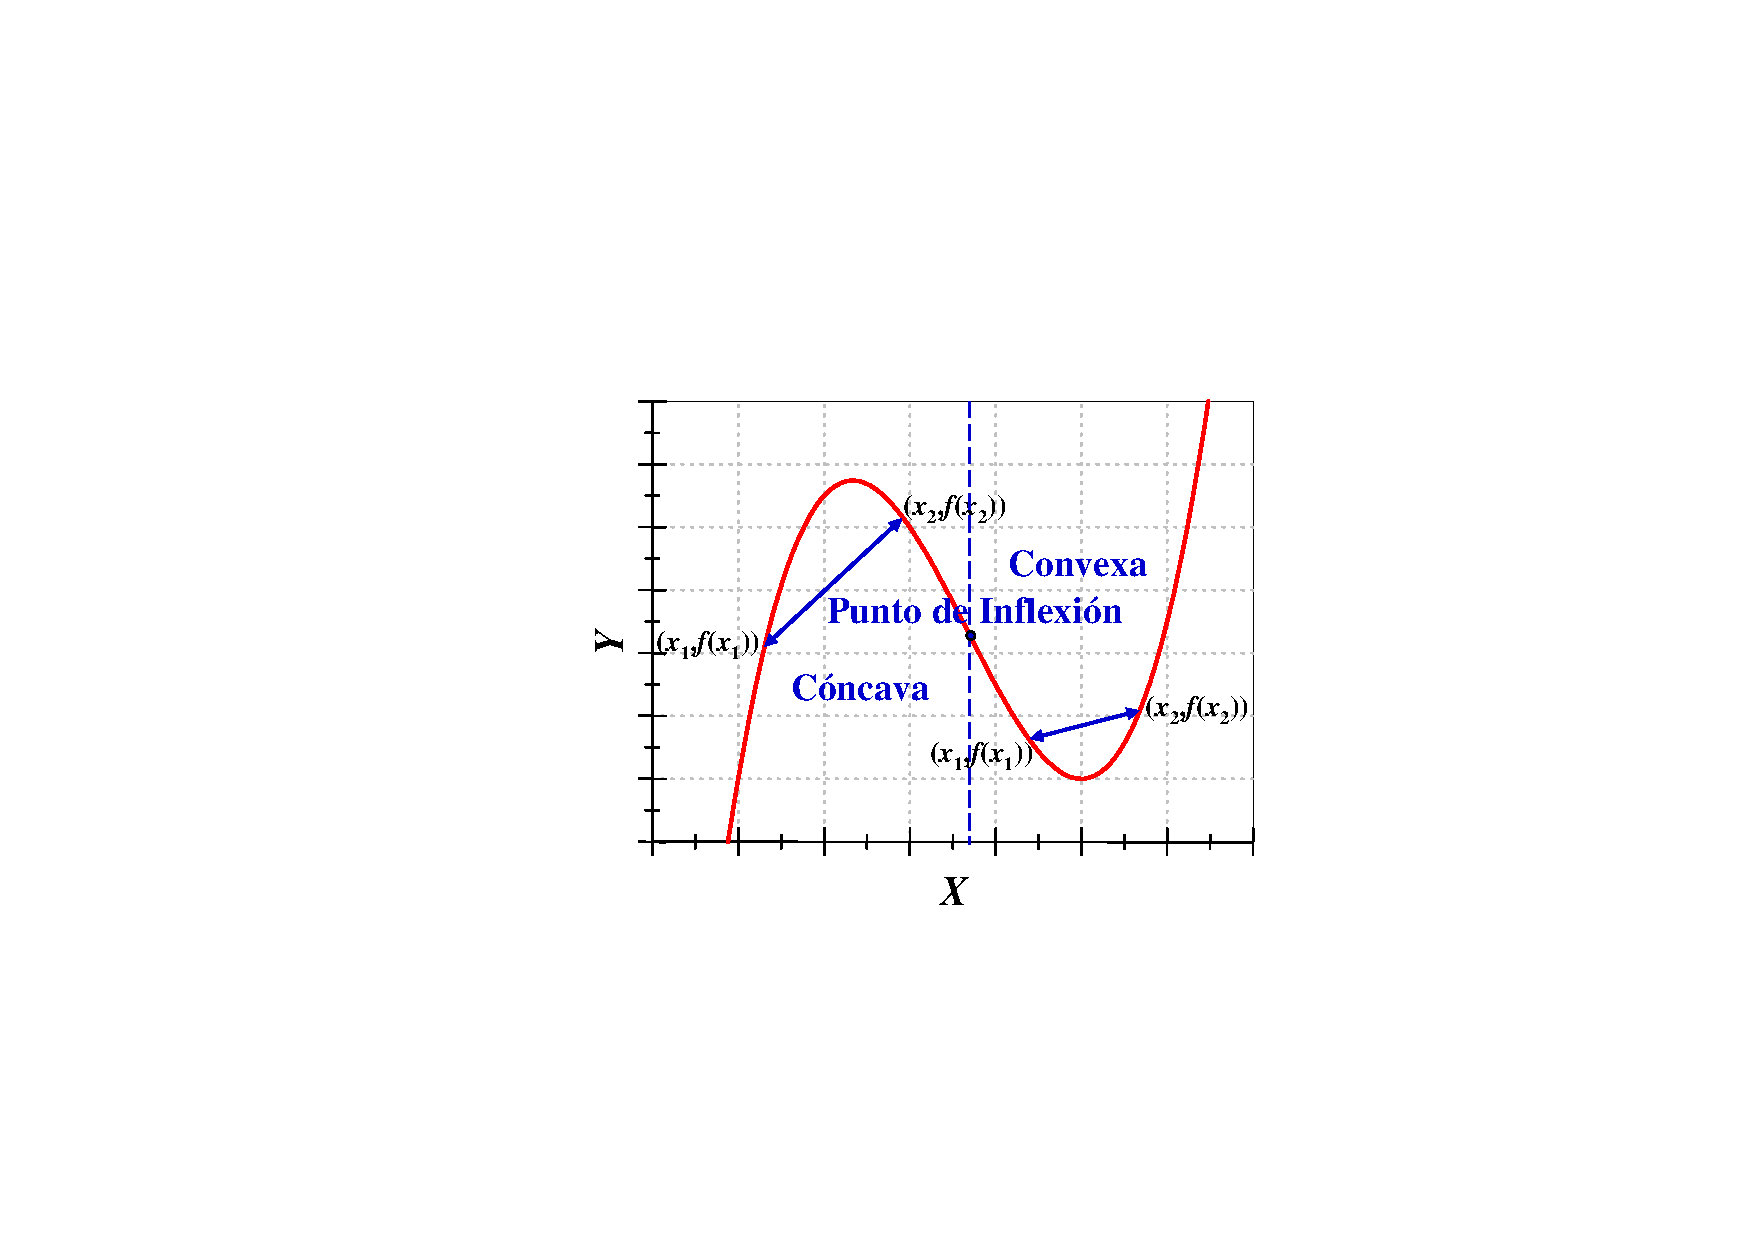
\includegraphics[scale=0.6]{concavidad}
\caption{Intervalos de concavidad y convexidad en una función.}
\label{g:concavidad}
\end{figure}


Si $f$ es una función derivable en el intervalo $I$, el signo de la segunda derivada puede utilizarse para estudiar la concavidad de la función ya que se cumple:
\begin{itemize}
\item $f$ es cóncava en $x_0\in I$, si y sólo si, $f''(x_0)\leq 0$.
\item $f$ es convexa en $x_0\in I$, si y sólo si, $f''(x_0)\geq 0$.
\end{itemize} 


\subsection*{Teorema del valor medio y teorema de Rolle}
Los siguientes teoremas nos proporcionan más aplicaciones de la derivada, como por ejemplo en el cálculo de las raíces de una función.

\begin{teorema}[Valor Medio]
Sea $f$ una función continua en el intervalo $[a,b]$ y derivable en $(a,b)$, entonces existe un valor $c\in(a,b)$ tal que 
\[
f'(c)=\frac{f(b)-f(a)}{b-a}=\frac{\Delta y}{\Delta x}
\]
\end{teorema}

Geométricamente, esto significa que existe algún punto $c\in(a,b)$ en el que la pendiente de la recta tangente a $f$ en el punto $(c,f(c))$ es igual a la pendiente de la recta secante a $f$ que pasa por los puntos $(a,f(a))$ y $(b,f (b))$, o lo que es lo mismo, ambas rectas son paralelas, tal y como se ve en la figura~\ref{g:teorema valor medio}.

\begin{figure}[h!]
\centering
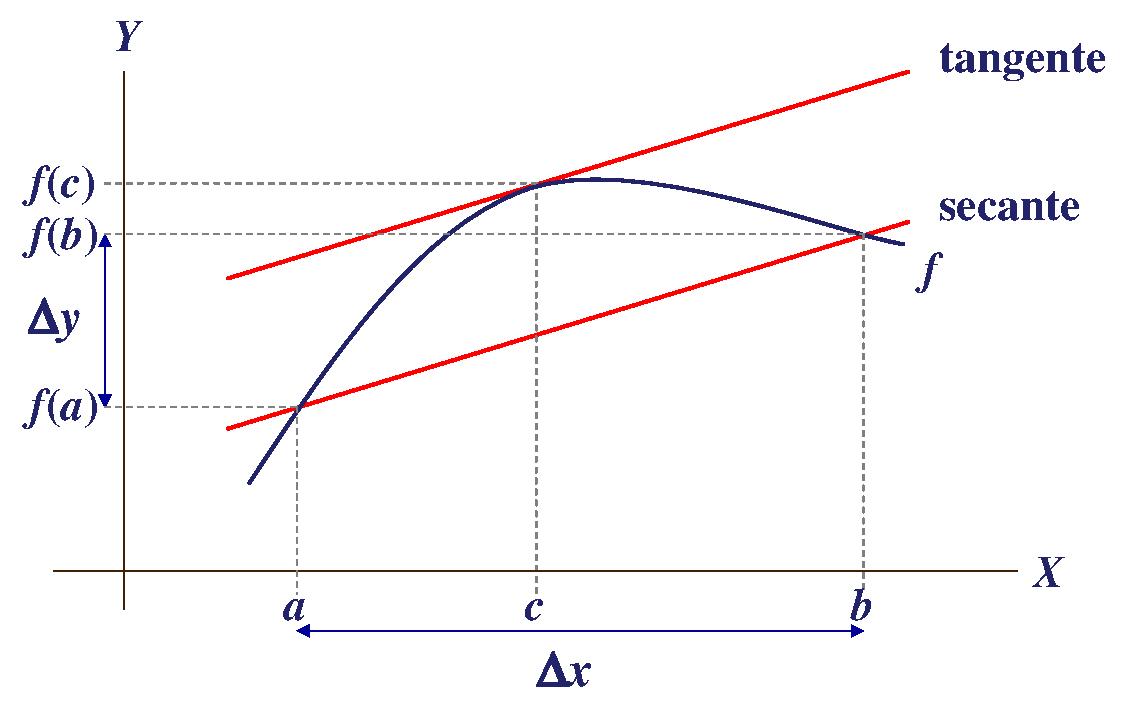
\includegraphics[scale=0.5]{teoremavalormedio}
\caption{Interpretación geométrica del teorema del valor medio.}
\label{g:teorema valor medio}
\end{figure}

Si pensamos el la derivada como en la tasa de variación instantánea de una función, entonces el teorema afirma que la tasa de variación media que experimenta $f$ sobre el intervalo $[a,b]$ es igual a la tasa de variación instantánea de $f$ en algún instante $c$ del intervalo $(a,b)$. Por ejemplo, si recorremos 10 km en una hora, entonces en algún momento habremos estado viajando exactamente a una velocidad de 10 km/h.

\begin{teorema}[Rolle]
Sea $f$  una función continua en el intervalo $[a,b]$ y derivable en $(a,b)$, tal que $f(a)=f(b)$. Entonces existe un valor $c\in(a,b)$ tal que $f'(c)=0$.
\end{teorema}

Este teorema es un caso particular del teorema del valor medio cuando se cumple que $f(a)=f(b)$.

Desde el punto de vista geométrico, el teorema asegura que entre dos puntos de igual ordenada de la gráfica de $f$, siempre existe algún punto con tangente horizontal, según se muestra en la figura~\ref{g:teorema rolle}.

\begin{figure}[h!]
\centering
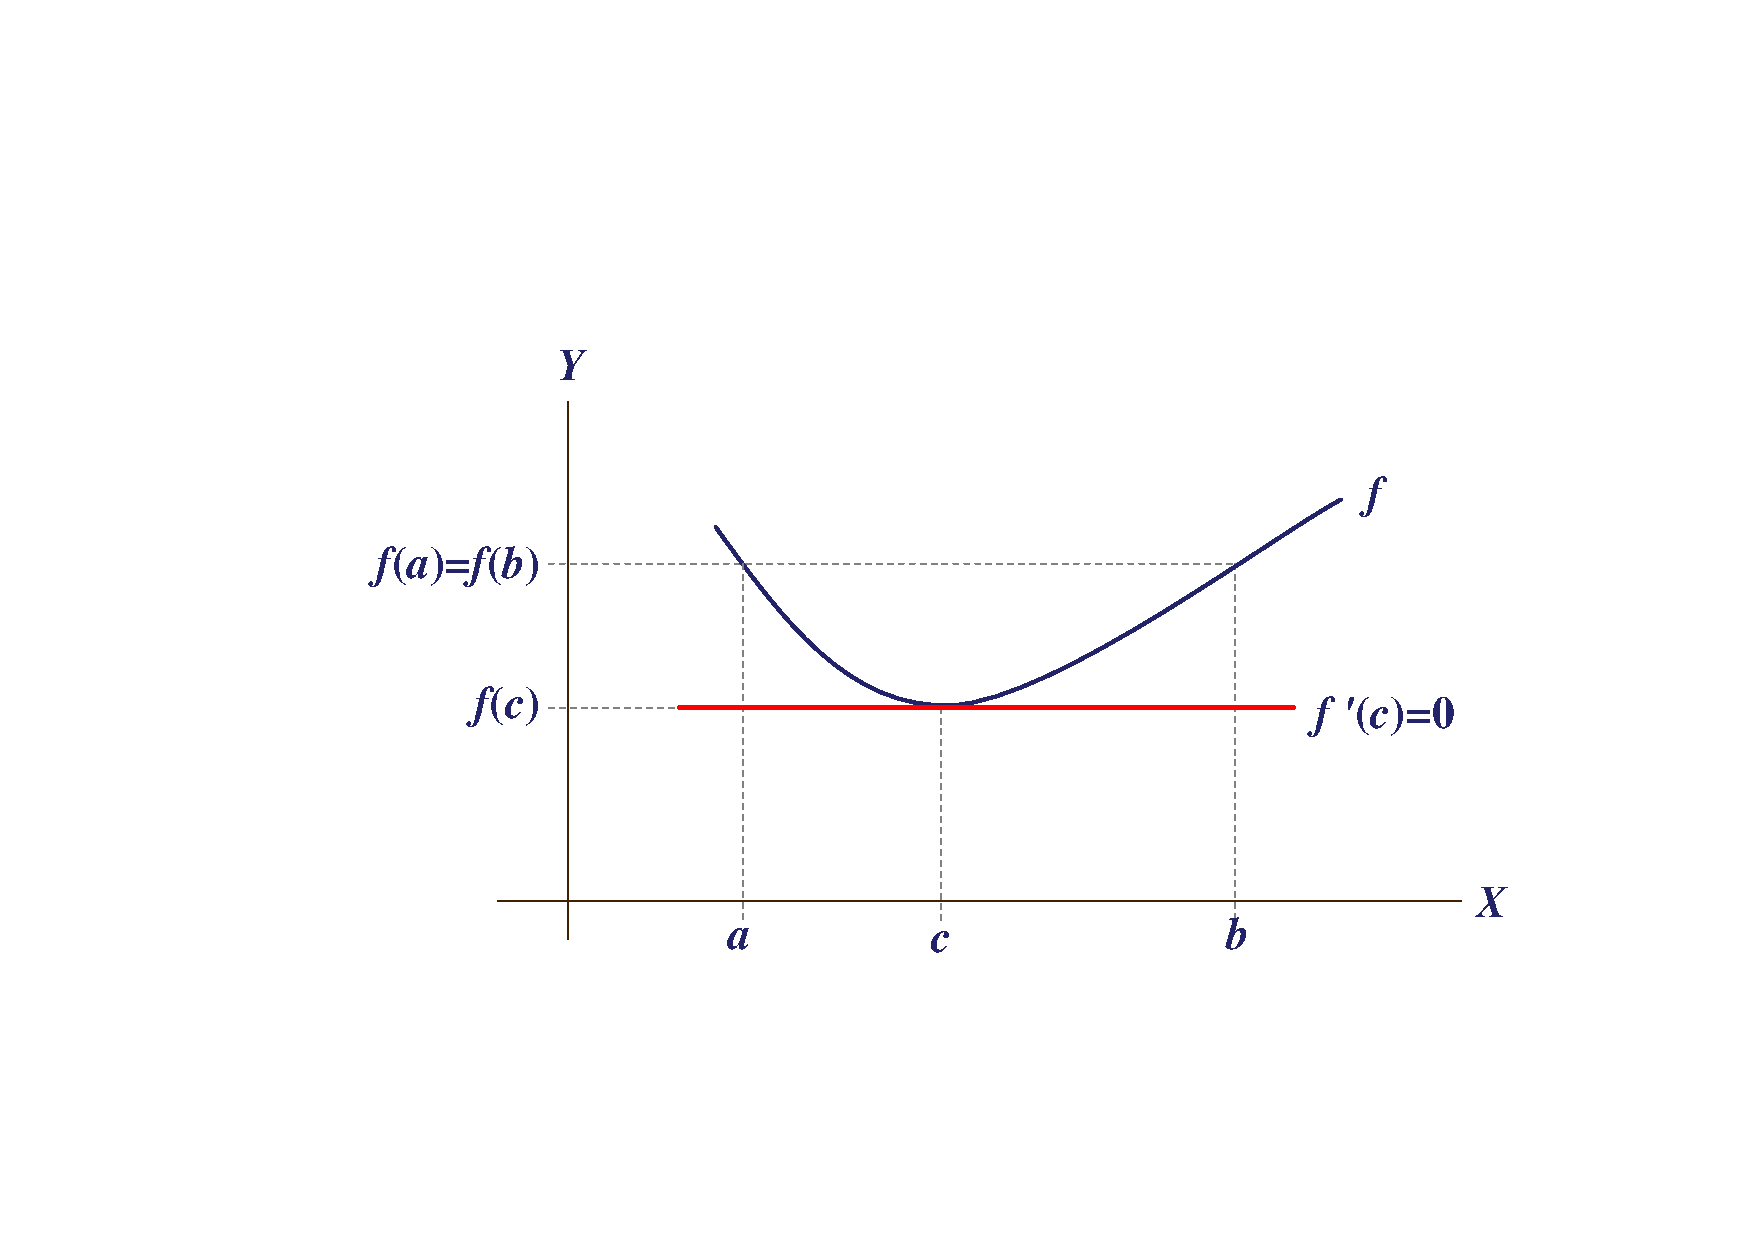
\includegraphics[scale=0.5]{teoremarolle}
\caption{Interpretación geométrica del teorema de Rolle.}
\label{g:teorema rolle}
\end{figure}

Si aplicamos el teorema para $f(a)=f(b)=0$, entonces el teorema asegura que entre dos raíces consecutivas de $f$ siempre se puede encontrar alguna raíz de su función derivada.

\section*{Ejercicios Prácticos}
\begin{enumerate}[leftmargin=*]
\item  Dada la función:
\[
g(x)=\dfrac{2x^{3}-3x}{x^{2}+1}
\]

\begin{enumerate}
\item  Representar la gráfica de $g$.

\item  Calcular la función derivada $g^{\prime }(x),$ y representar su
gráfica.

\item  Calcular las raíces de $g^{\prime }(x).$

\item  A la vista de las raíces y de la gráfica de la función
derivada, determinar los extremos relativos de la función y los
intervalos de crecimiento.

\item Calcular la segunda derivada $g''(x),$ y representar su
gráfica.

\item  Calcular las raíces de $g''(x).$

\item  A la vista de las raíces y de la gráfica de la segunda
derivada, determinar los intervalos de concavidad de la función y los puntos de inflexión.
\end{enumerate}

\item Estudiar el crecimiento, la concavidad, los extremos relativos y los puntos de inflexión de la función $f(x)=\dfrac{x}{x^2-2}$.

\item  Demostrar que la ecuación $e^x=1-x$ tiene exactamente
una solución real, aplicando el teorema de Rolle.

\item  A las cuatro de la tarde un coche pasa, a una velocidad de 70
km/h por el punto kilométrico 400 de la autopista $A4$. Diez
minutos después pasa, circulando a una velocidad de 80 km/h, por
el punto kilométrico 425 de la citada autopista. Le para la
policía y le pone una multa por exceso de velocidad. Suponiendo que la velocidad máxima permitida es de 120 km/h, 
¿tenía razón la policía?
\end{enumerate}

\section*{Problemas}
\begin{enumerate}[leftmargin=*]

\item Estudiar el crecimiento, la concavidad, los extremos relativos y los puntos de inflexión de la función $f(x)=\log(x^2+1)$.

\item  Demostrar que para cualquier valor de $k\in \mathbb{R}$ la
ecuación $x^3-3x+k=0$ no puede tener dos raíces en el
intervalo $(0,1)$.

\item  En el movimiento uniformemente acelerado de ecuación
$x=8t^2-2t+5$ se puede asegurar, durante el intervalo de tiempo
[0,1], que la velocidad media coincide con la velocidad
instantánea en un cierto momento $t_{0}$. Calcular $t_{0}$.
¿Qué propiedad nos asegura la certeza de la proposición
anterior?
\end{enumerate}

\end{document}
